\documentclass[times]{article}

\usepackage[margin=1.0in]{geometry}
\usepackage{graphicx}
\usepackage{adjustbox}
\usepackage{float}
\usepackage{placeins}
\usepackage[none]{hyphenat}
\usepackage{amsmath}
\usepackage[us]{datetime}
\usepackage[explicit]{titlesec}
\begin{document}
	\title{Dalton Cole \\ drcgy5@mst.edu \\ COMP SCI 5401 FS2017 Assignment 1b}
	\date{\formatdate{24}{9}{2017}}
	\maketitle

	\section{Average vs Best Fitness}
	As can be seen from Figure \ref{fig:graph_1}, the designed EA gradually improves as the number of evaulations goes up. This is what is expected from evolutionary algorithms. This trend does not continue in Figure \ref{fig:graph_2} and Figure \ref{fig:graph_3}. The solution improves rapidly at first, but quickly levels off.
	
	\begin{figure}
		\caption{Average and Best Fitness for Input 1}
		\label{fig:graph_1}
		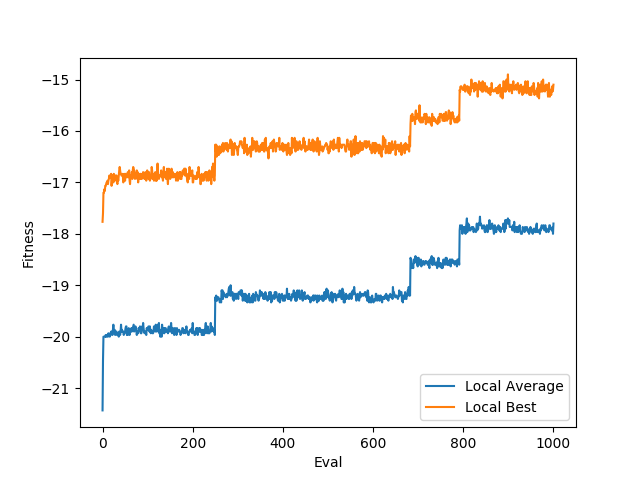
\includegraphics[width=\textwidth]{../graphs/1.png}
	\end{figure}

	\begin{figure}
		\caption{Average and Best Fitness for Input 2}
		\label{fig:graph_2}
		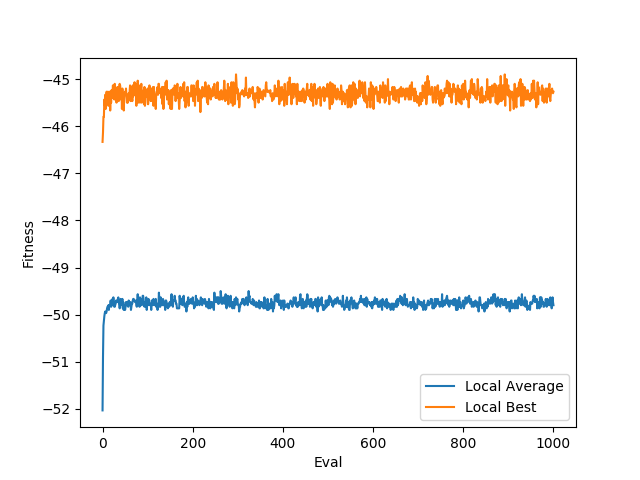
\includegraphics[width=\textwidth]{../graphs/2.png}
	\end{figure}

	\begin{figure}
		\caption{Average and Best Fitness for Input 3}
		\label{fig:graph_3}
		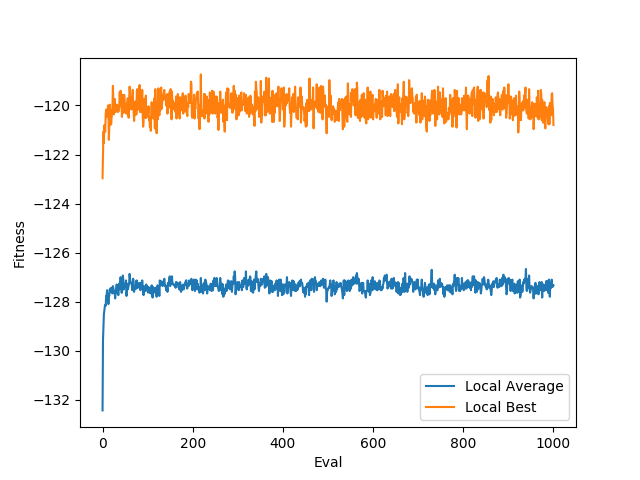
\includegraphics[width=\textwidth]{../graphs/3.png}
	\end{figure}

	\section{1A vs 1B}
	F and t tests are employed to test the null hypotheses that both random search and evolutionary algorithms (EA) produce equally good results. This is because the distribution is not known, but 30 runs are completed for each test case.

	\subsection{First Input}
	As can be seen from Figure \ref{fig:f_test1}, a t-test with equal variance is used because the mean of random search is less than the mean of EA and F $>$ F Critical one-tail. In Figure \ref{fig:t_test1} shows that T-stat is less than t Critical two-tail, so the null hypothesis is not rejected and there is NO SIGNIFICANT DIFFERENCE between the two algorithms.

	\subsection{Second Input}
	As can be seen from Figure \ref{fig:f_test2}, a t-test with unequal variance is used because the mean of random search is less than the mean of EA and F $<$ F Critical one-tail. In Figure \ref{fig:t_test2} shows that T-stat is less than t Critical two-tail, so the null hypothesis is not rejected and there is NO SIGNIFICANT DIFFERENCE between the two algorithms.

	\subsection{Third Input}
	As can be seen from Figure \ref{fig:f_test3}, a t-test with equal variance is used because the mean of random search is less than the mean of EA and F $<$ F Critical one-tail. In Figure \ref{fig:t_test3} shows that T-stat is less than t Critical two-tail, so the null hypothesis is not rejected and there is NO SIGNIFICANT DIFFERENCE between the two algorithms.


	\begin{figure}
		\caption{F Test for Input 1 Assignment 1B vs 1A}
		\label{fig:f_test1}
		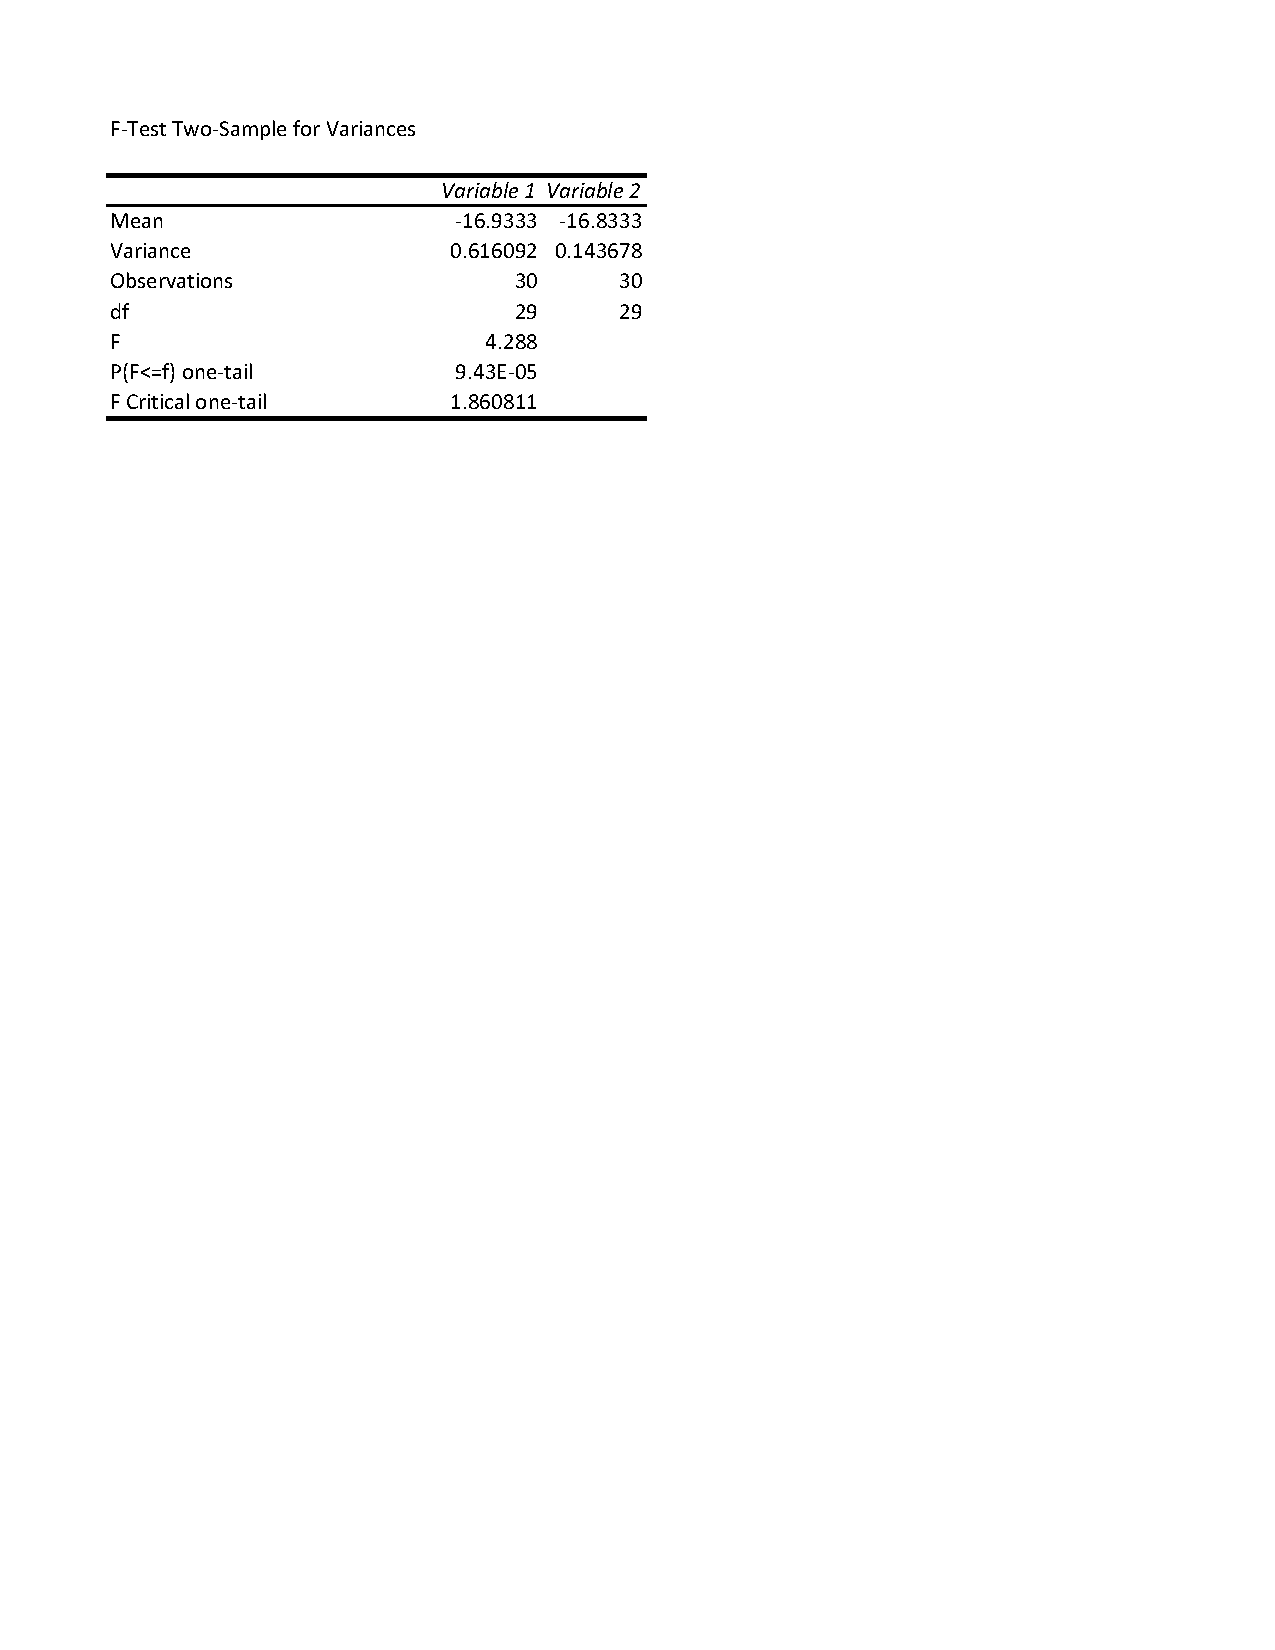
\includegraphics[width=\textwidth]{./tests/Input1_f_test.pdf}
	\end{figure}

	\begin{figure}
		\caption{T Test for Input 1 Assignment 1B vs 1A}
		\label{fig:t_test1}
		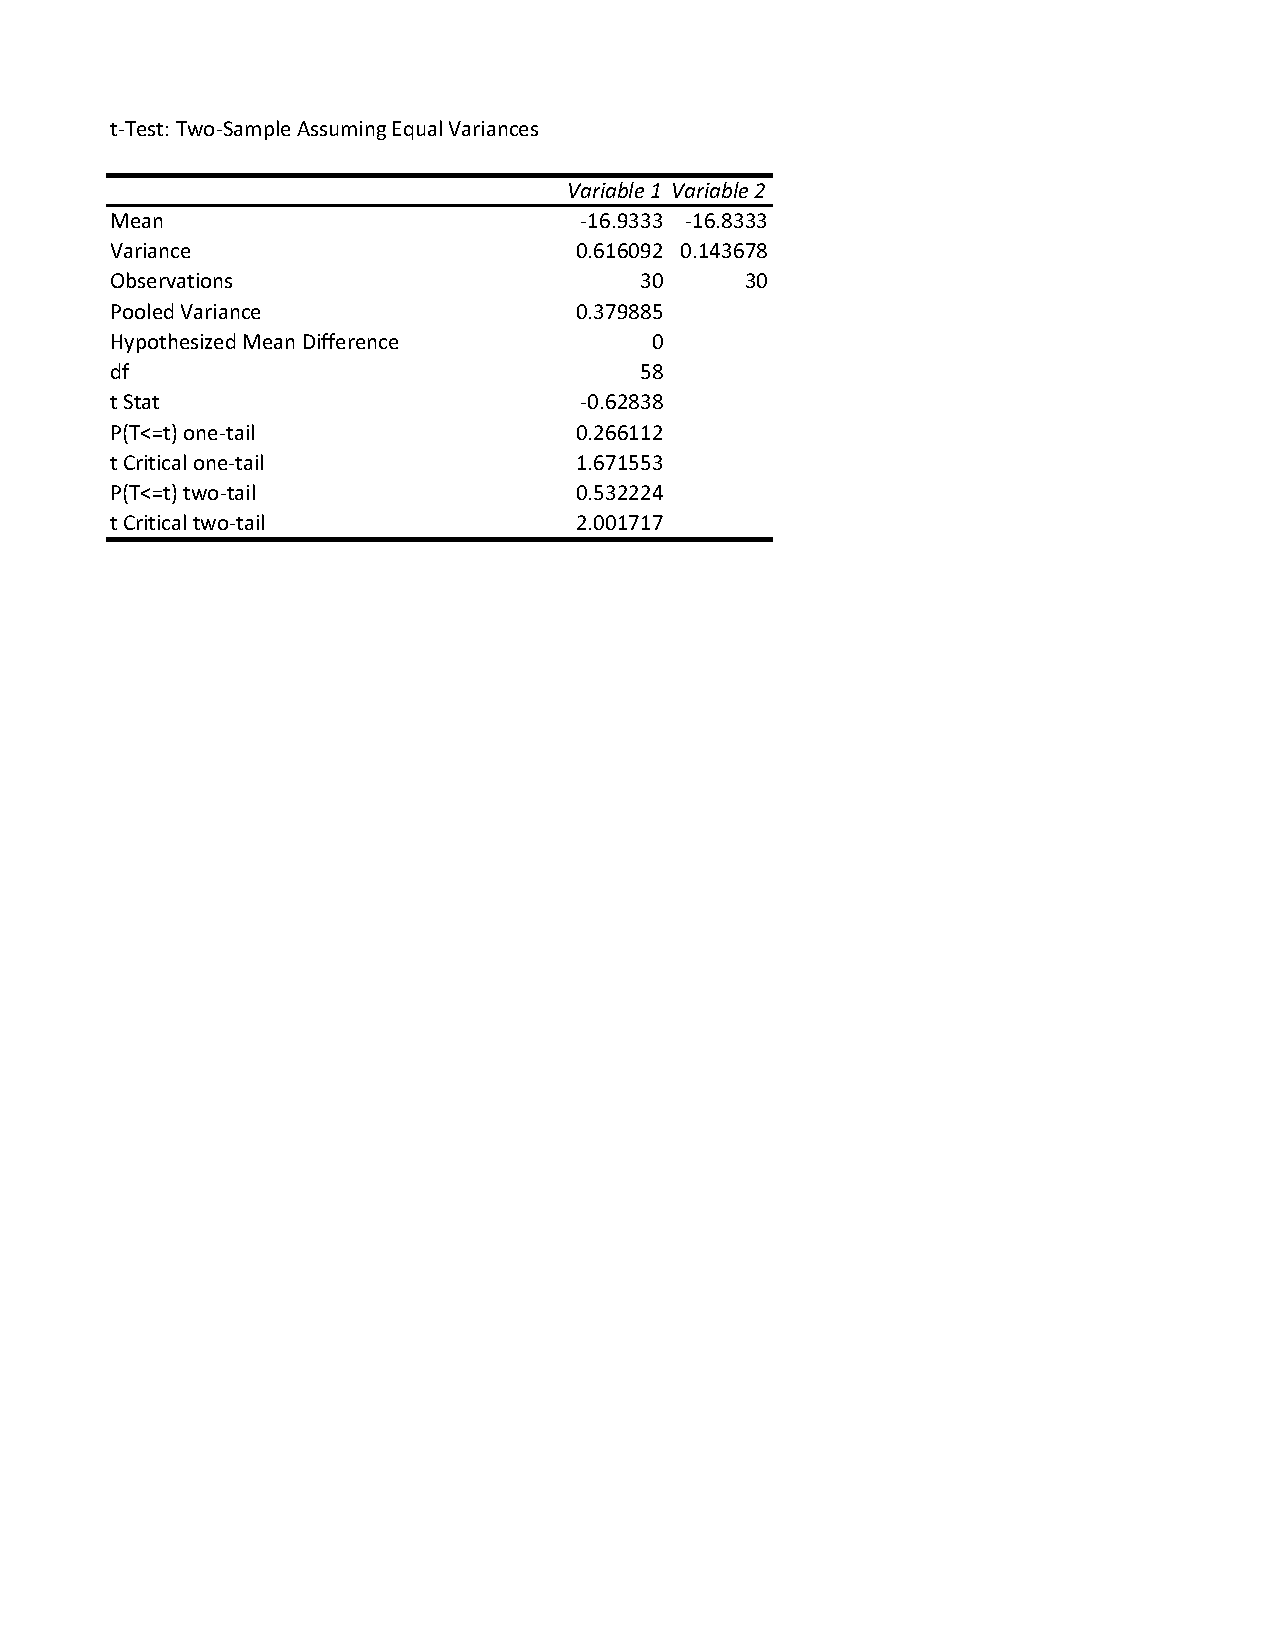
\includegraphics[width=\textwidth]{./tests/Input1_t_test.pdf}
	\end{figure}

	\begin{figure}
		\caption{F Test for Input 2 Assignment 1B vs 1A}
		\label{fig:f_test2}
		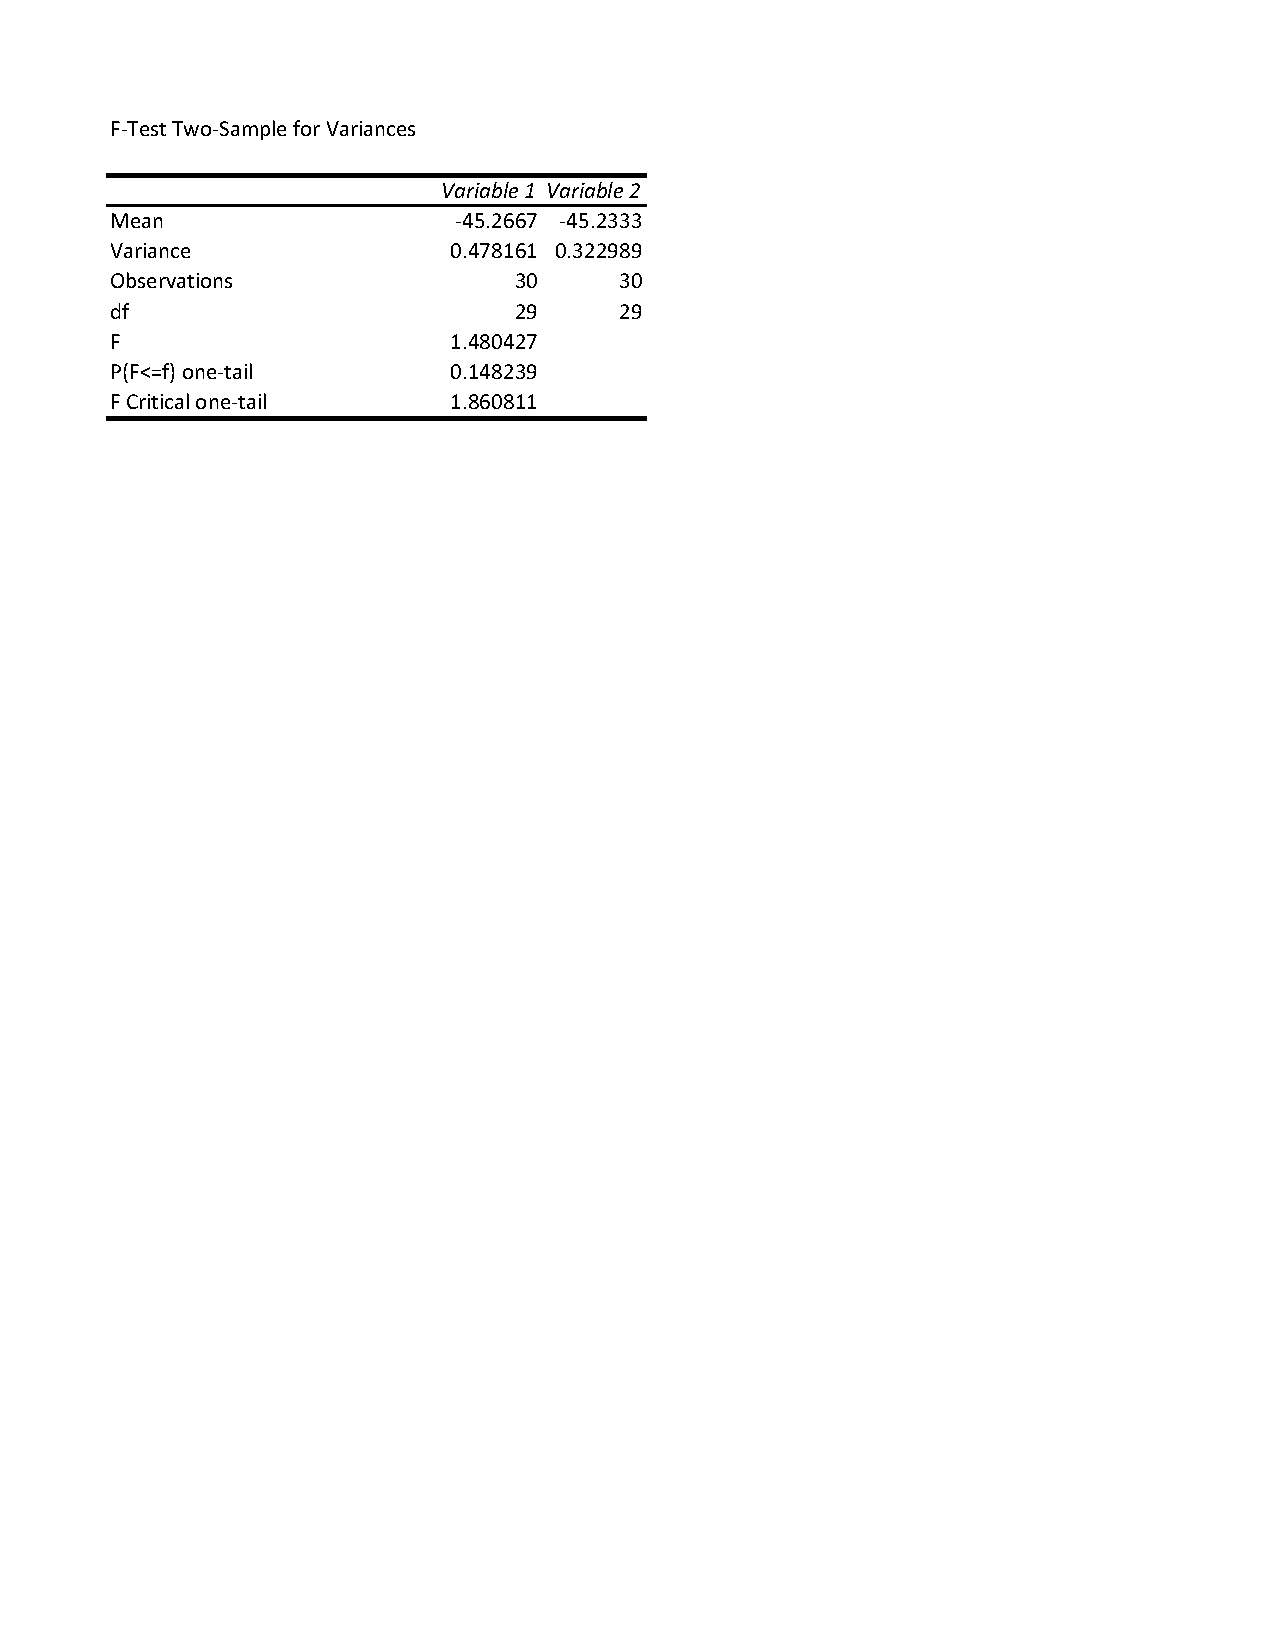
\includegraphics[width=\textwidth]{./tests/Input2_f_test.pdf}
	\end{figure}

	\begin{figure}
		\caption{T Test for Input 2 Assignment 1B vs 1A}
		\label{fig:t_test2}
		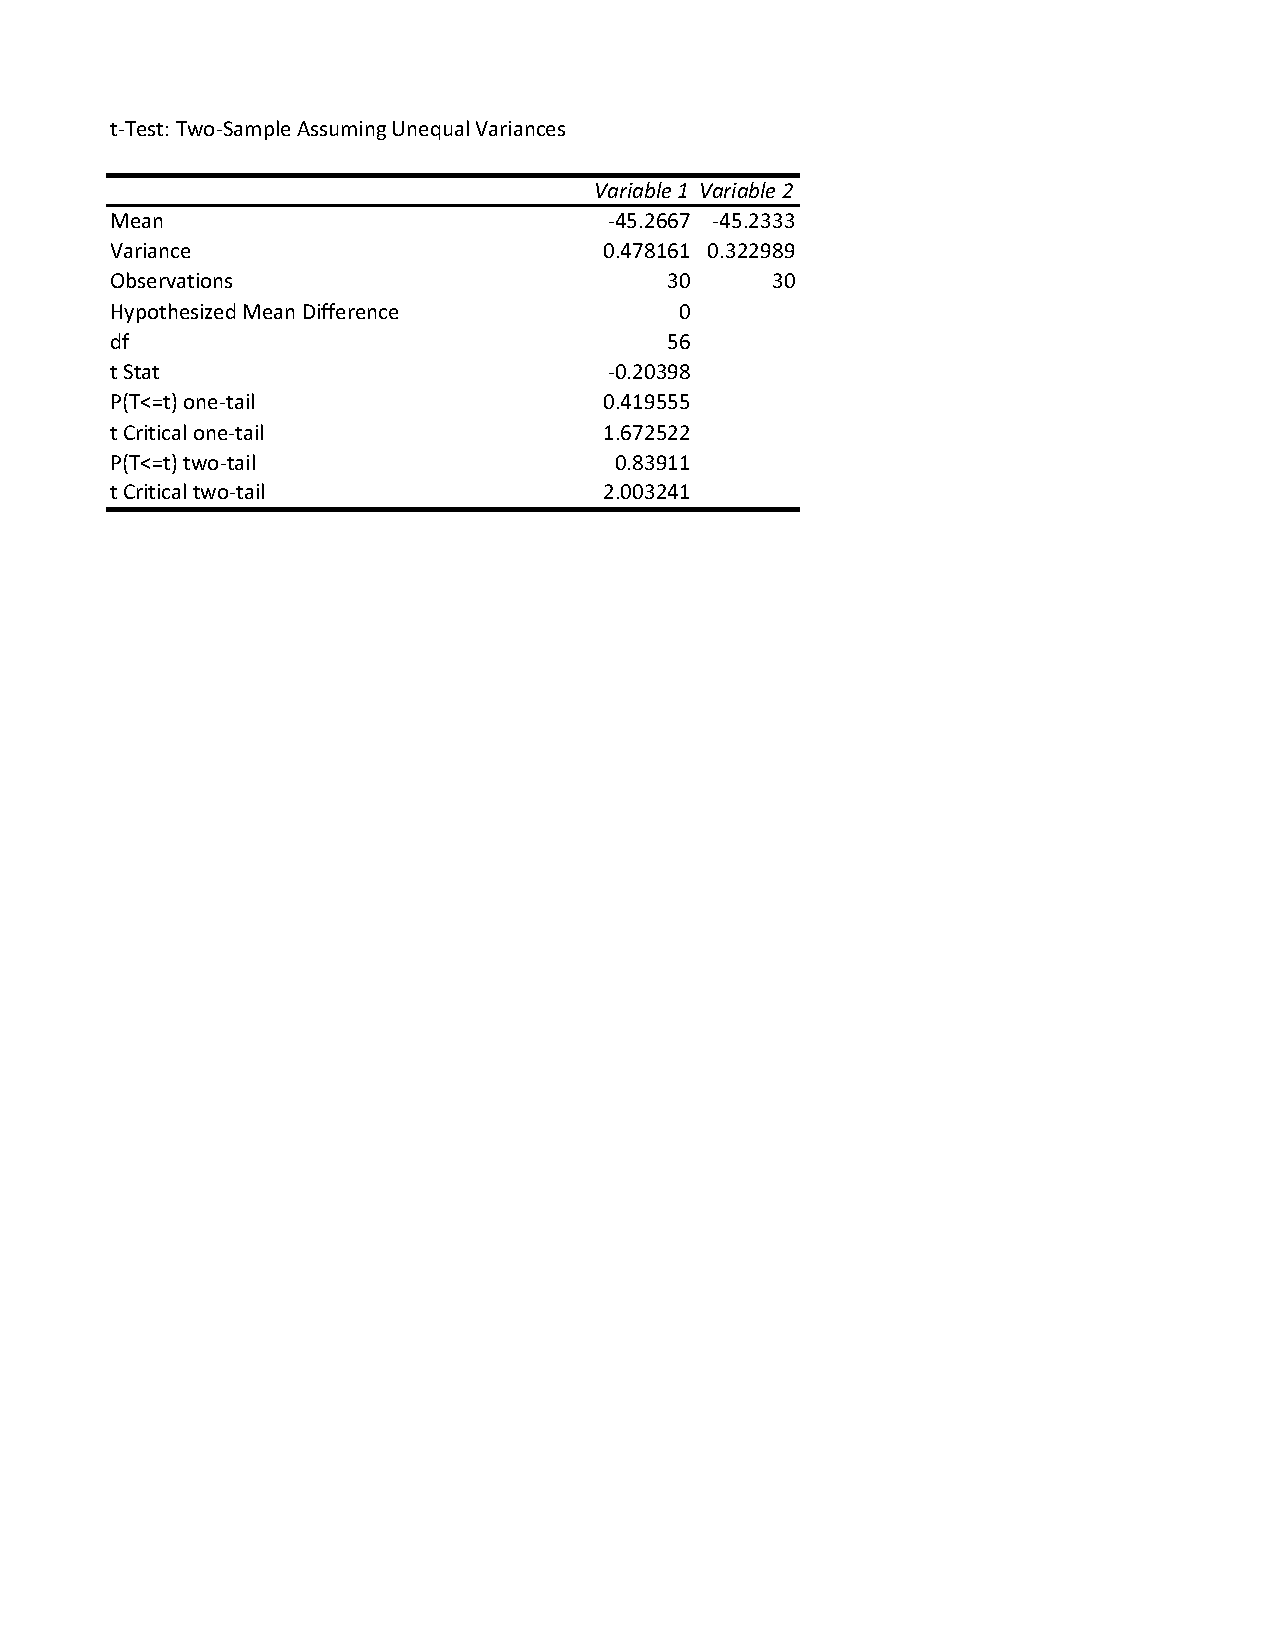
\includegraphics[width=\textwidth]{./tests/Input2_t_test.pdf}
	\end{figure}

	\begin{figure}
		\caption{F Test for Input 3 Assignment 1B vs 1A}
		\label{fig:f_test3}
		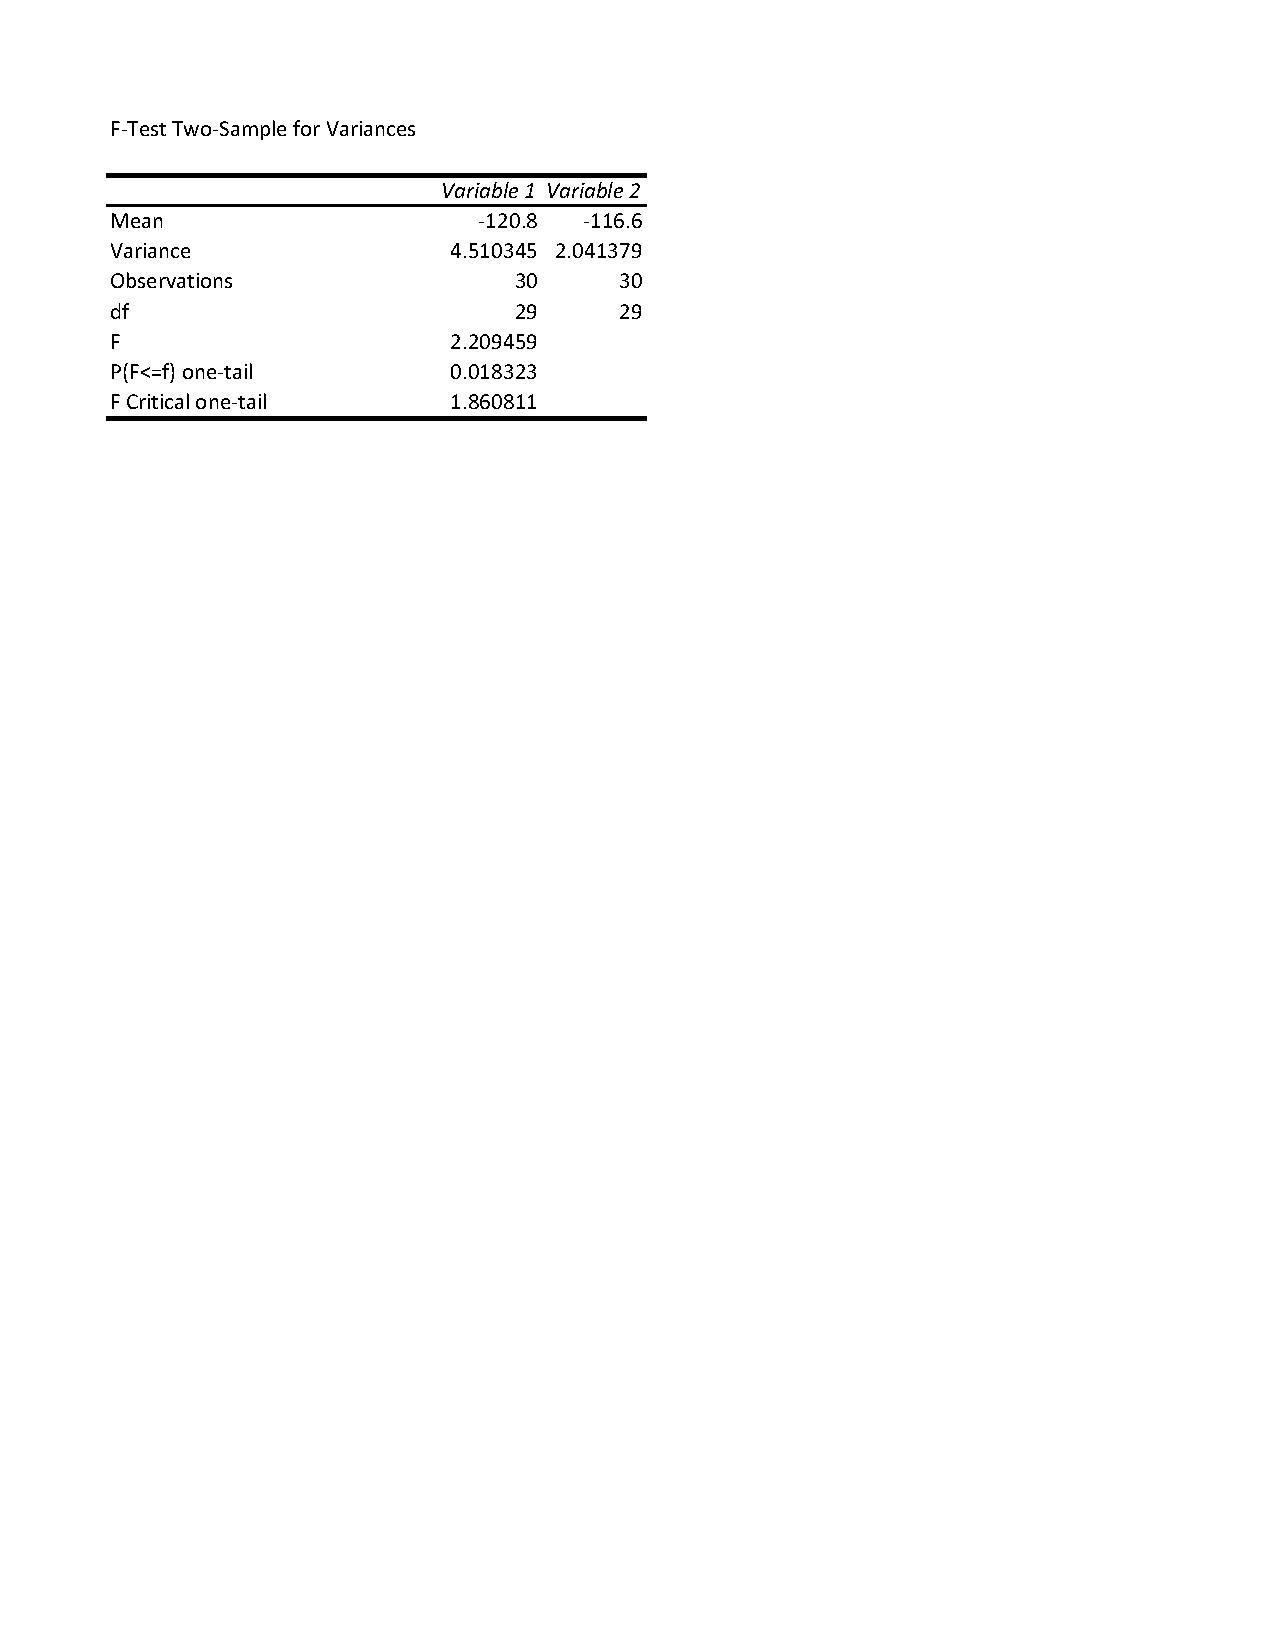
\includegraphics[width=\textwidth]{./tests/Input3_f_test.pdf}
	\end{figure}

	\begin{figure}
		\caption{T Test for Input 3 Assignment 1B vs 1A}
		\label{fig:t_test3}
		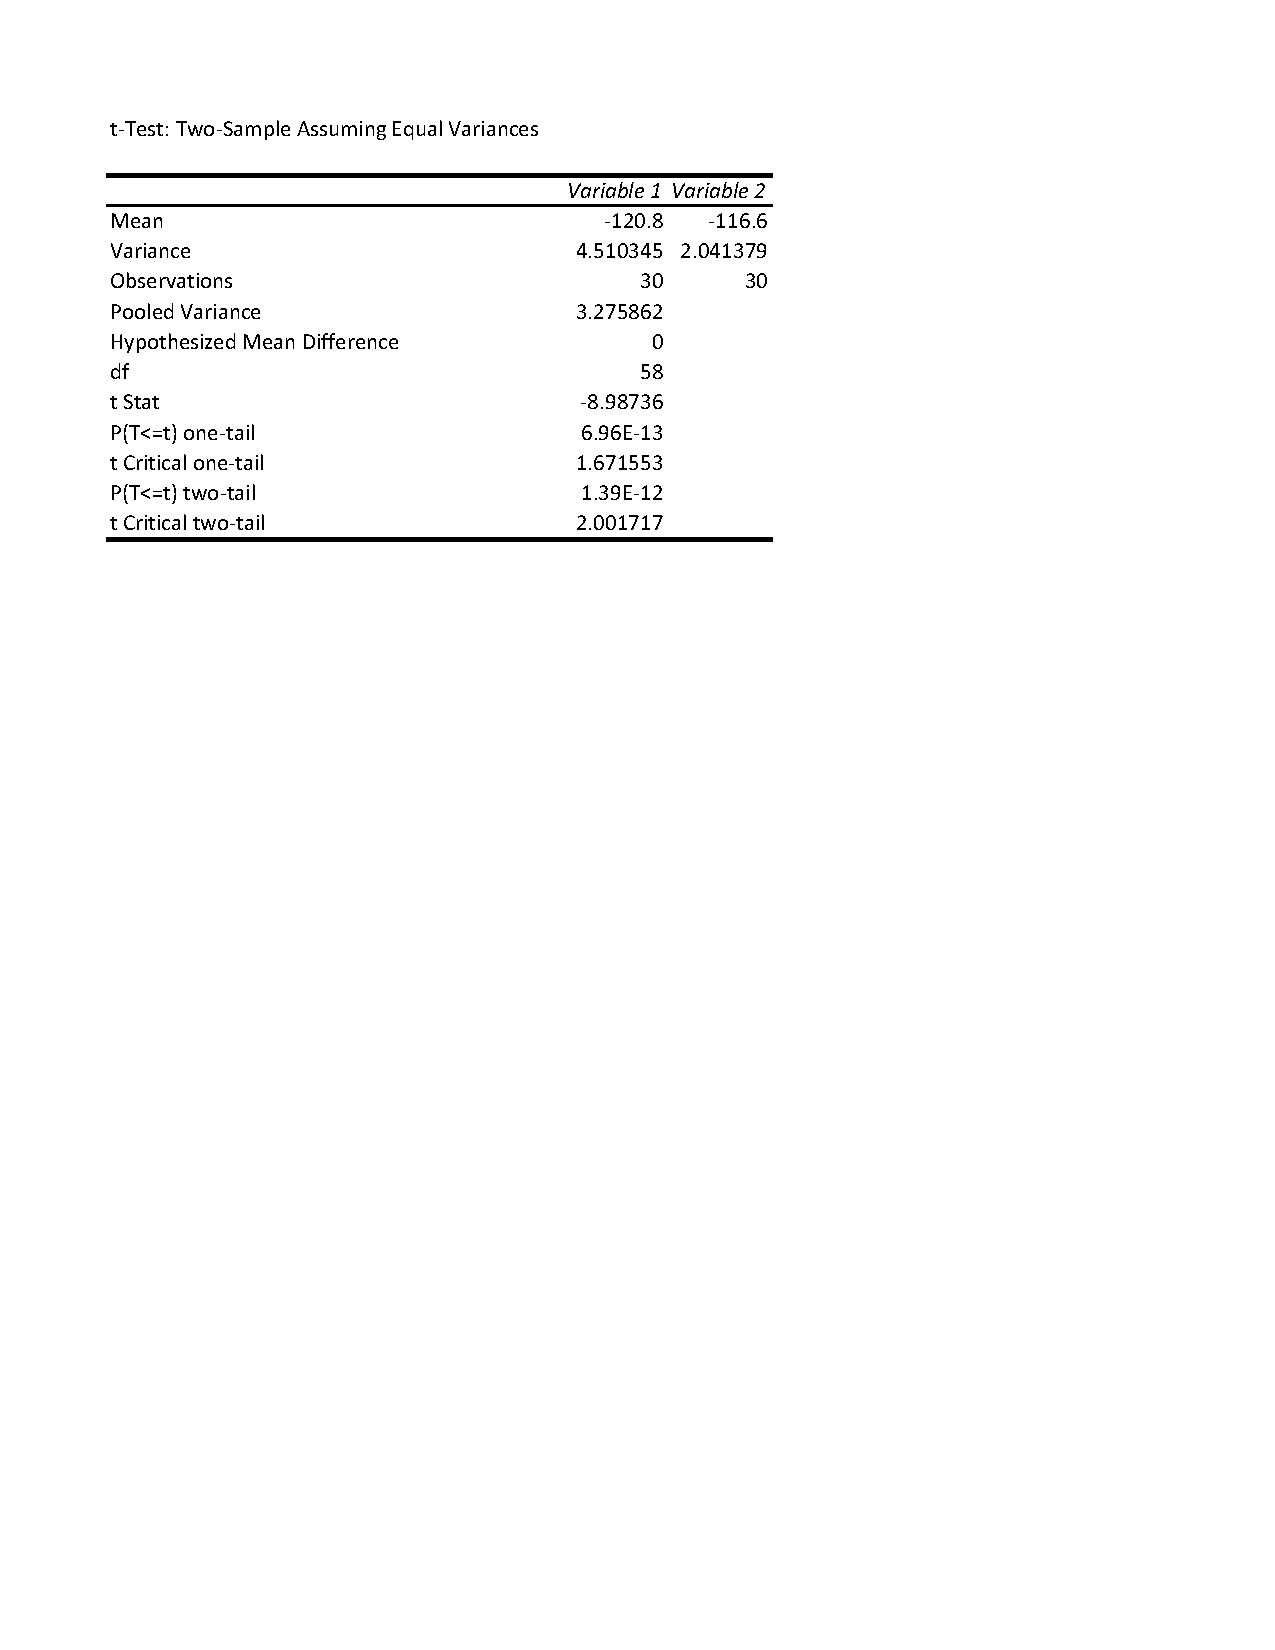
\includegraphics[width=\textwidth]{./tests/Input3_t_test.pdf}
	\end{figure}
		
\end{document}